\documentclass[letterpaper]{article}

\usepackage{graphicx}
\usepackage{mathtools}
\usepackage{enumerate}
\usepackage[letterpaper,left=1.25in,right=1.25in,top=1in,bottom=1in]{geometry}
\usepackage{fancyhdr}
\usepackage[parfill]{parskip}
\usepackage{changepage}

\pagestyle{fancy}
\fancyfoot{}
% header/footer settings
\lhead{Kevin Nash (kjn33)}
\chead{EECS 391 -- P2}
\rhead{\today}
\cfoot{\thepage}

\begin{document}

\section{Linear Decision Boundaries}

\subsection{Plotting Iris Classes}
This project is written in Python, using Pandas dataframes to manipulate data
and Matplotlib to plot it.

The data is initialized like so,
\begin{verbatim}
# Read the file into a Pandas dataframe
iris_data = pd.read_csv(filename)
# Capitalize the column names and remove underscores
iris_data.columns = ["Sepal Length", "Sepal Width", "Petal Length",
                     "Petal Width", "Species"]
# Remove any species other than those specified by the assignment
iris_data = iris_data.loc[iris_data["Species"].isin(["versicolor", "virginica"])]
# Select the versicolor and virginica species individually
versi_data = iris_data.loc[iris_data["Species"] == "versicolor"]
virgi_data = iris_data.loc[iris_data["Species"] == "virginica"]
\end{verbatim}
The assignment asks us to consider only the versicolor and virginica species.
Let's take a look at the first few rows of each.
\begin{verbatim}
In [2]: versi_data.head(3)
    Sepal Length  Sepal Width  Petal Length  Petal Width     Species
50           7.0          3.2           4.7          1.4  versicolor
51           6.4          3.2           4.5          1.5  versicolor
52           6.9          3.1           4.9          1.5  versicolor

In [3]: virgi_data.head(3)
     Sepal Length  Sepal Width  Petal Length  Petal Width    Species
100           6.3          3.3           6.0          2.5  virginica
101           5.8          2.7           5.1          1.9  virginica
102           7.1          3.0           5.9          2.1  virginica
\end{verbatim}
We are interested in the petal dimensions. To plot them:
\begin{verbatim}
fig = plt.figure()
ax = fig.add_subplot(111)
ax.scatter(x=dataset_1["Petal Length"], y=dataset_1["Petal Width"],
           color="b", marker="o", label="versicolor")
ax.scatter(x=dataset_2["Petal Length"], y=dataset_2["Petal Width"],
           color="r", marker="^", label="virginica")
plt.xlabel("Petal Length (cm)")
plt.ylabel("Petal Width (cm)")
plt.legend(loc="upper left")
plt.savefig("plot_1a.pdf", bbox_inches="tight")
\end{verbatim}
This gives us
\begin{center}
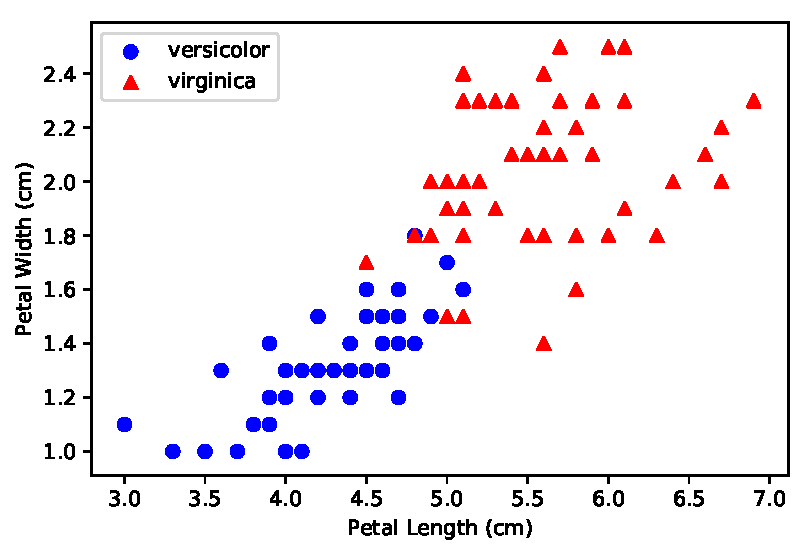
\includegraphics{plot_1a.pdf}
\end{center}
It is clear that at least two points of different classes overlap, which means
that our data is not going to be linearly separable.

\subsection{Choosing a Boundary by Hand}

I chose a boundary by physically drawing a line on the above plot using an
image editor. The line reaches from 2.4 on the y-axis to 6.5 on the x-axis.
Then we can get an equation in slope-intercept form from the coordinates
$(3, 2.4), (6.5, 1)$. $y=mx+b$ where $m=-0.4$ and $b=3.6$.

The code to generate this plot is identical to the above plot, except the line
\begin{verbatim}
plt.plot([3, 6.5], [2.4, 1], color="k", linestyle="-", linewidth=1)
\end{verbatim}
is now added before saving.
\begin{center}
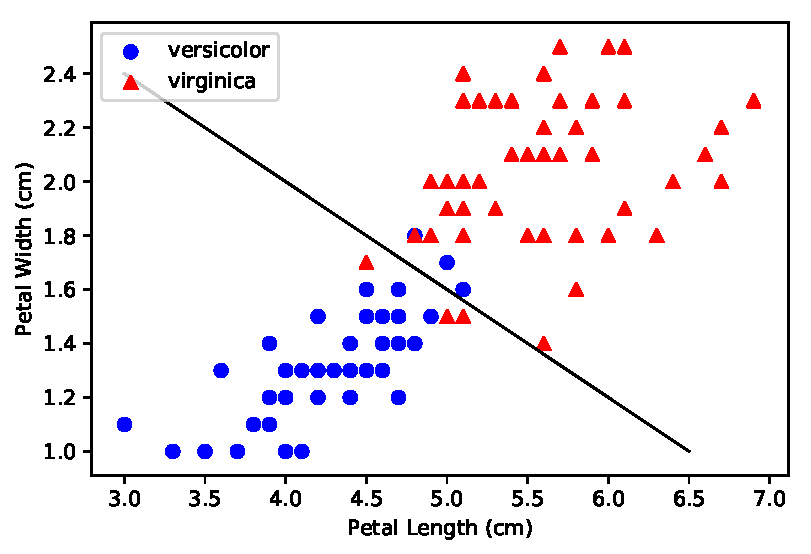
\includegraphics{plot_1b.pdf}
\end{center}

\subsection{Defining a Threshold Classifier}

We can now define a threshold classifier using the above parameters to compare
against our data points. Simply put, if the point is above the line, it is
predicted to be virginica. Otherwise it is predicted to be versicolor.

The calculation is shown here, where $x$ and $y$ correspond to $petal\ length$
and $petal\ width$, respectively.
\begin{verbatim}
""" Returns the distance from point (x,y) to the line in slope-intercept form """
def dist_from_line(x, y, m, b):
    return y - (m * x + b)

""" Returns "virginica" if the point (length, width) is above the line """
def classify_linear(row, slope, intercept):
    if 0 < dist_from_line(row["Petal Length"], row["Petal Width"], slope, intercept):
        return "virginica"
    return "versicolor"
\end{verbatim}

To plot this data, we isolate the misclassified points into their own dataframes.
Misclassified points are defined as those for which $Species \neq Classification$.
\begin{verbatim}
# Classify data linearly for part 1c
iris_data["Classification"] = iris_data.apply(
    lambda row: classify_linear(row, -0.4, 3.6), axis=1
)
misclassified = pd.DataFrame(columns=iris_data.columns)

for i, row in iris_data.iterrows():
    if not row["Classification"] == row["Species"]:
        misclassified.loc[len(misclassified.index)] = row

print("Linear decision accuracy: {}%".format(100 - len(misclassified.index) /
      len(iris_data.index) * 100))

versi_class = misclassified.loc[misclassified["Species"] == "versicolor"]
virgi_class = misclassified.loc[misclassified["Species"] == "virginica"]
plot_linear_bound(versi_class, virgi_class, "plot_1c.pdf")
\end{verbatim}
This threshold classifier misclassifies six data points, as shown in the next
plot. Note that points \textit{above} the line are supposed to be virginica
(red triangles), and points \textit{below} the line are supposed to be
versicolor (blue circles), but the opposite is true of misclassified points.
\begin{center}
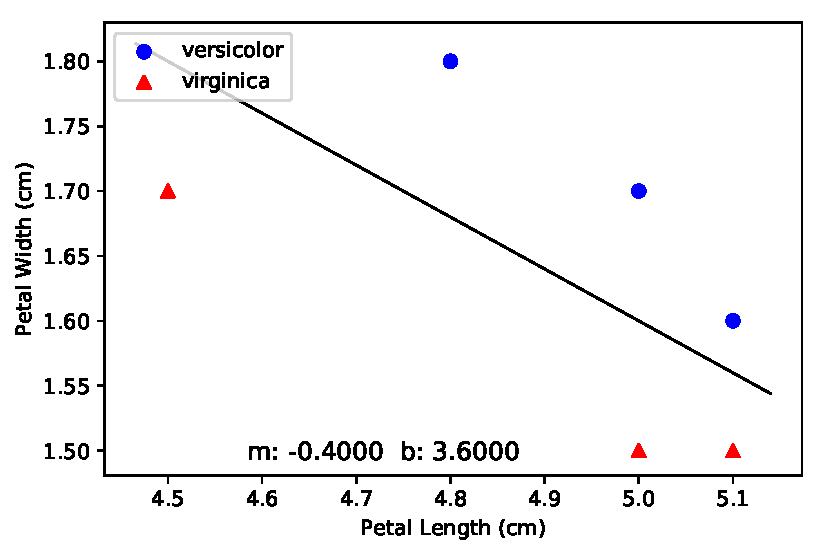
\includegraphics{plot_1c.pdf}
\end{center}

\subsection{Circle Decision Boundaries}

Instead of defining our decision boundary with a straight line, we can use
a circle instead. The technique is the same, although in this case the decision
is made considering whether a point is inside or outside of the circle, rather
than above or below a line. The functions are similar to those first shown in
section 1.3.
\begin{verbatim}
""" Returns the distance from point (x,y) to the edge of the circle """
def dist_from_circle(x, y, x_circ, y_circ, r):
    return ((x - x_circ)**2 + (y - y_circ)**2)**0.5 - r

""" Returns "virginica" if the point (length, width) is outside of the circle """
def classify_circular(row, x, y, radius):
    if 0 < dist_from_circle(row["Petal Length"], row["Petal Width"], x, y, radius):
        return "virginica"
    return "versicolor"
\end{verbatim}
Now we need to pick parameters for our circle ($x_{0}, y_{0}, r$). The
assignment instructs us to pick three sets. I started at the center of the plot
with an arbitrary radius of $\frac{1}{2}$. This, predictably, didn't give great
results, but with two adjustments the decision accuracy eventually met that of
the linear threshold ($94\%$). The parameters and results are shown below,
followed by the plot of each. Note that because the $x,y$ scales are not $1:1$,
the circle is \textit{mathematically} circular, \textit{not graphically} circular.
\begin{center}
\begin{tabular}{|c|c|c|c|}
\hline
$x$ & $y$ & $r$ & Accuracy\\
\hline\hline
$4.75$ & $1.7$ & $0.5$ & 58\%\\
\hline
$4.5$ & $1.2$ & $0.5$ & 79\%\\
\hline
$4.0$ & $1.2$ & $1$ & 94\%\\
\hline
\end{tabular}
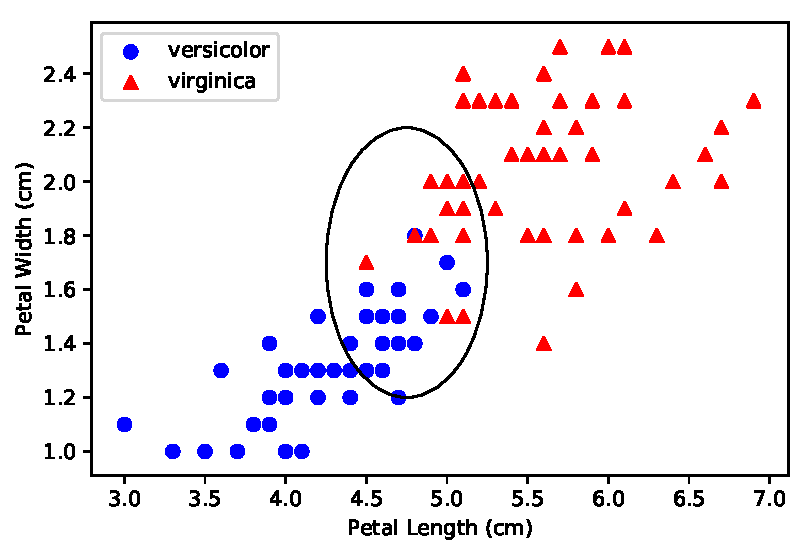
\includegraphics{plot_1d_1.pdf}
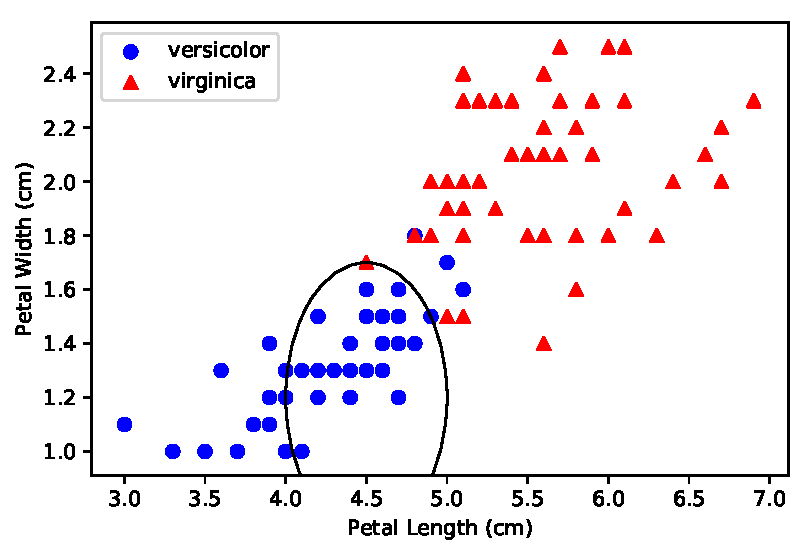
\includegraphics{plot_1d_2.pdf}
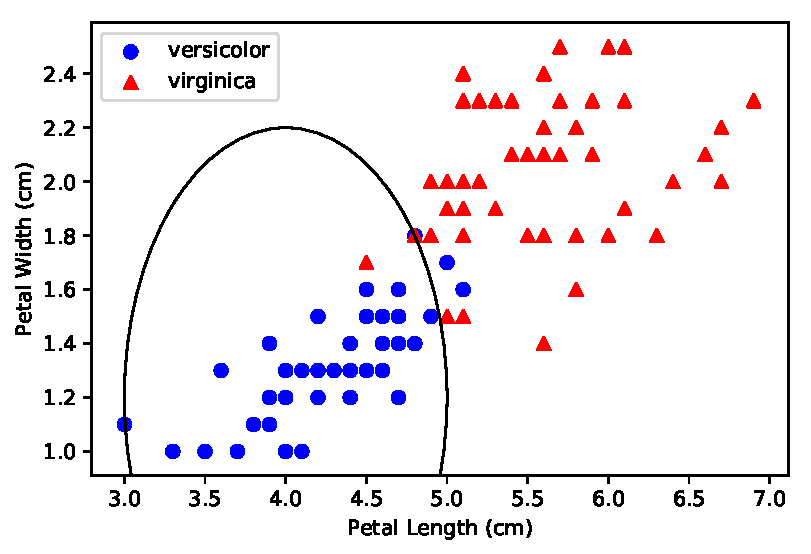
\includegraphics{plot_1d_3.pdf}
\end{center}

The plotting code is easy to imagine. Instead of drawing a line, just draw
a circle according to
\begin{verbatim}
circle = plt.Circle((x, y), r, color="k", fill=False)
ax.add_artist(circle)
\end{verbatim}

\section{Objective Functions}

\subsection{Calculating Mean-Squared Error}

The mean squared error is given by
\begin{equation*}
E = \frac{1}{N}\sum_{n=1}^N\left(\boldsymbol{w}^T\boldsymbol{x}_n-c_n\right)^2
\end{equation*}
In our case the predicted and actual values are $\boldsymbol{w}^T\boldsymbol{x}_n$
and $c_n$, where class of $x$ in pattern vector $\boldsymbol{x}_n$ is given by
\[
    x \in
    \begin{cases}
    \text{class 1} & \text{if } y\geq 0\\
    \text{class 2} & \text{if } y < 0
    \end{cases}
\]
and we can number the classes $0$ or $1$ to give $c_n$ a value according to
\[
    c_n =
    \begin{cases}
    0 & \boldsymbol{x}_n \in \text{class 1}\\
    1 & \boldsymbol{x}_n \in \text{class 2}
    \end{cases}
\]
However by this definition, $(\boldsymbol{x}_n-c_n)\subset \{-1,0,1\}$ and
therefore $(\boldsymbol{x}_n-c_n)^2\subset \{0,1\}$. The mean of zeroes and
ones doesn't give us a very percise error value, and so we can redefine the
first term. Rather than assigning a zero or a one based on the predicted class,
we can plug distance into a modified version of the sigmoid function, shown
below.
\begin{equation*}
p = \frac{1}{1+10^{-d}}
\end{equation*}
where $d$ is the distance from the decision boundary and $p$ is the predictive
value. $p\in[0,1]$, which changes the prediction from a discrete set of one and
zero to a continuum from zero to one. By making this change, we qualify our
predictions with a degree of confidence and theoretically make our MSE value
more accurate.

From now on the MSE value will be superimposed over the graph. The current
boundary gives a value of $0.0645$.
\begin{center}
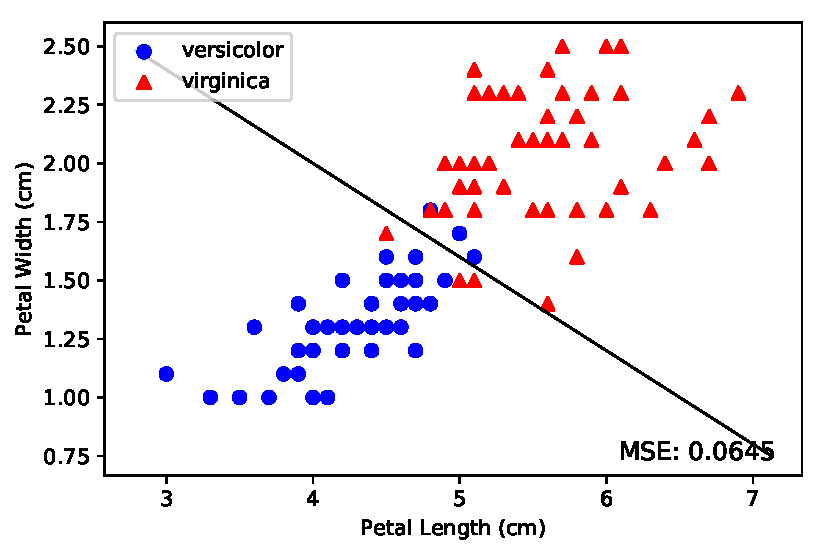
\includegraphics{plot_2a.pdf}
\end{center}
\begin{verbatim}
if show_mse:
    combined_data = pd.concat([dataset_1, dataset_2])
    mse = mean_squared_error(combined_data, slope, intercept)
    plt.text(0.85, 0.05, "MSE: %.4f" % mse, ha='center', va='center',
             fontsize=12, transform=ax.transAxes)
\end{verbatim}
The mean squared error calculation is calculated like so
\begin{verbatim}
def mean_squared_error(dataset, m, b, classes={"versicolor": 0, "virginica": 1}):
    sum_diffs = 0
    for i, row in dataset.iterrows():
        dist = dist_from_line(m=m, b=b, row=row)
        sum_diffs += (classes[row["Species"]] -
            classes[classify_prediction(dist)] * sigmoid(dist))**2
    return sum_diffs / len(dataset.index)

def sigmoid(x):
    return 1 / (1 + 10**(-x))
\end{verbatim}
 
\subsection{Examples of Large and Small Errors}

As was shown in the previous section, the MSE value for a line with $m=-0.4$, $b=3.6$ was
quite small ($0.0645$). We can generate a large MSE value ($0.6862$) by using a positive
slope. Here the boundary misclassifies the majority of the data points!
\begin{verbatim}
# Very high MSE
plot_linear_bound(versi_data, virgi_data, 1.5, -5.5, show_mse=True, filename="plot_2b_1.pdf")
\end{verbatim}
\begin{center}
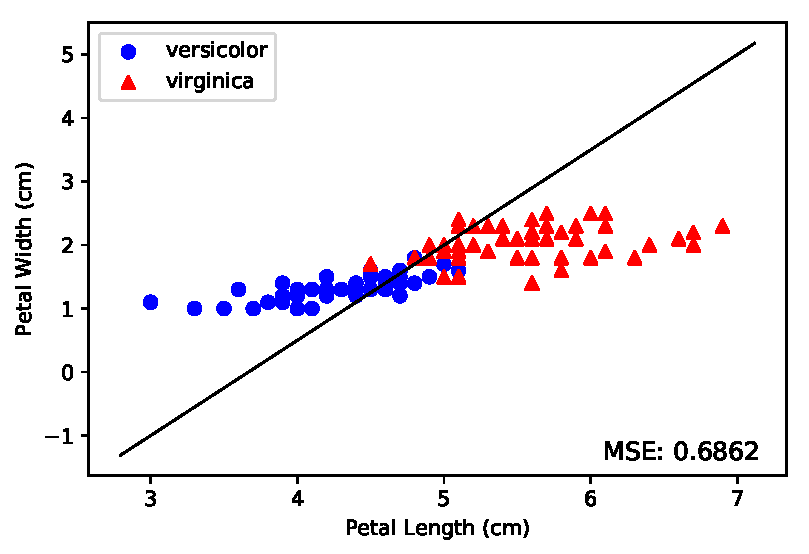
\includegraphics{plot_2b_1.pdf}
\end{center}
To lower the MSE, we should move our parameters back to their ``approximately optimal''
values. Let's see what a zero slope about halfway through the data gives us.
\begin{verbatim}
# Lower MSE
plot_linear_bound(versi_data, virgi_data, 0, 1.65, show_mse=True, filename="plot_2b_2.pdf")
\end{verbatim}
\begin{center}
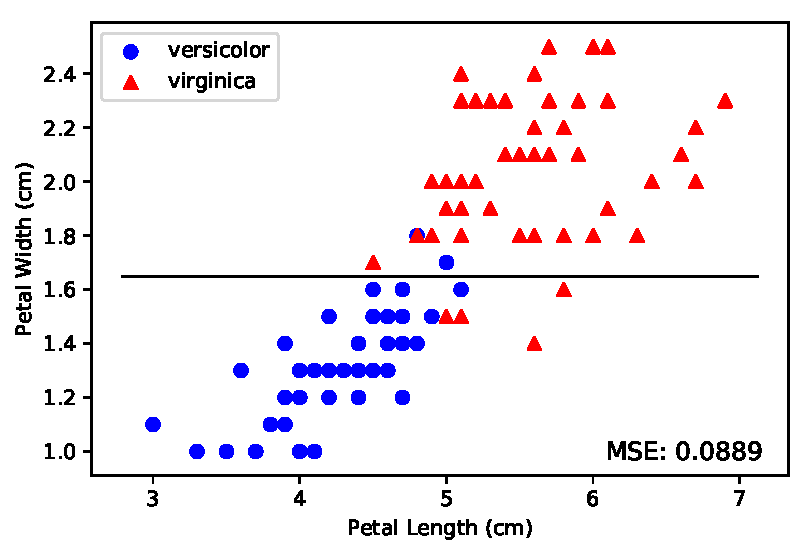
\includegraphics{plot_2b_2.pdf}
\end{center}
$0.0889$ is much closer to our original value of $0.0645$.

\subsection{Derivation of the Gradient}

Starting with the mean square equation from section 2.1,
\begin{equation*}
E = \frac{1}{N}\sum_{n=1}^N\left(\boldsymbol{w}^T\boldsymbol{x}_n-c_n\right)^2
\end{equation*}
Where $E$ is the mean-squared error, $N$ is the number of data points (in this
case 100), $\boldsymbol{w}^T$ is the vector of weights, $\boldsymbol{x}_n$ is
the vector of data point classifications, and $c_n$ is its actual class (in
this case species).

As was previously stated, I am improving the error function with a modified
sigmoid curve. The distance value supplied to that function is calculated with
\begin{equation*}
d = W_n - (w_1 \cdot L_n + w_2)
\end{equation*}
where $W_n$ is the petal width, $L_n$ is the petal length, $w_1$ is the first
weight corresponding to slope, $w_2$ is the second weight corresponding to
intercept.

The modified sigmoid function is then used to get a bias term ($w_0$).
\begin{equation*}
w_0 = S(d) = \frac{1}{1+10^{-d}}
\end{equation*}
The derivative of this sigmoid function is
\begin{equation*}
S'(d) = S(d)\cdot(1-S(d))\cdot\text{ln}|10|
\end{equation*}

If we combine these equations, the MSE equation is written
\begin{equation*}
E = \frac{1}{N}\sum_{n=1}^N\left(S(W_n - (w_1 \cdot L_n + w_2))\cdot\boldsymbol{x}_n-c_n\right)^2
\end{equation*}
The gradient for this MSE involves differentiating its equation, as is done below.
\begin{equation*}
\begin{split}
\frac{\partial E}{\partial\boldsymbol{w}} &= \frac{2}{N}(1-S(\boldsymbol{x}\boldsymbol{w}))(S(\boldsymbol{x}\boldsymbol{w})-\boldsymbol{c})\boldsymbol{x}\\
&= \frac{2}{N}(1-\boldsymbol{p})(\boldsymbol{p}-\boldsymbol{c})\boldsymbol{x}
\end{split}
\end{equation*}
At the end we replace the sigmoid function call with a vector of the predictive
values that it returns, notated $\boldsymbol{p}$.

This is the vector form. The scalar form will be shown in the next section.

\subsection{Gradients in Scalar and Vector Form}

We can expand the vector form of the gradient into a scalar form.
When expanded, it looks like:
\begin{equation*}
\text{Scalar:\quad} \frac{\partial E}{\partial w_i} = \frac{2}{N}\sum_{n=1}^N(x_{i,n}\cdot(1-S(x_n w)\cdot(S(x_n w)-c_n))
\end{equation*}
\begin{equation*}
\frac{2}{N}\sum_{n=1}^N(w_0x_{0,n}+\ldots+w_ix_{i,n}+\ldots+w_Mx_{M,n}-c_n)x_{i,n}
\end{equation*}
In this form the expression is summed over $N$ terms. The vector form is similar but
does not feature the summation, since it is implicit from the use of vectors
instead of scalar variables (e.g. $x_{i,n}$ and $\boldsymbol{x}$).
\begin{equation*}
\text{Vector:\quad} \frac{\partial E}{\partial\boldsymbol{w}} = \frac{2}{N}(1-S(\boldsymbol{x}\boldsymbol{w}))(S(\boldsymbol{x}\boldsymbol{w})-\boldsymbol{c})\boldsymbol{x}
\end{equation*}
Then to update the weight, we use an iteration function:
\begin{equation*}
w_i^{t+1}=w_1^t-\varepsilon\frac{\partial E}{\partial w_i}
\end{equation*}
Epsilon here is a small value that ensure we eventually converge on a minimum value.
At this point the difference between one MSE and the MSE of the next step is
negligible.

\subsection{Summing the Gradient for an Ensemble of Patterns}

We can now use a gradient to take steps that should ultimately minimize mean
squared error. To do this, we simply combine the tools outlined above.
Namely, we need the predictive function by which to compare the relative
confidence in each categorization, and the derivative, which tells us how to
improve this confidence (thereby lowering MSE).

\begin{verbatim}
def sum_gradient(dataset, m, b, classes={"versicolor": 0, "virginica": 1}):
    epsilon = 0.1 / len(dataset.index)
    gradient = 0
    for i, row in dataset.iterrows():
        pred = sigmoid(dist_from_line(m=m, b=b, row=row))
        error = pred - classes[row["Species"]]
        gradient += (2 / len(dataset.index)) * (1 - pred) * error
    if m < 0:
        new_m = m + epsilon * gradient
    else:
        new_m = m - epsilon * gradient
    new_b = b - epsilon * gradient
    return new_m, new_b
\end{verbatim}

The above function calculates the new slope and intercept for weights in the
next step in a gradient descent. Below are function calls to plotting routines
that produce the following plots. The plots show sequential steps (magenta)
from an initial decision boundary (black, dashed).

\begin{verbatim}
plot_gradient_descent(versi_data, virgi_data, -0.1, 5, snapshots=5, filename="plot_2e_1.pdf")
plot_gradient_descent(versi_data, virgi_data, -0.5, 3, snapshots=5, filename="plot_2e_2.pdf")
\end{verbatim}
\begin{center}
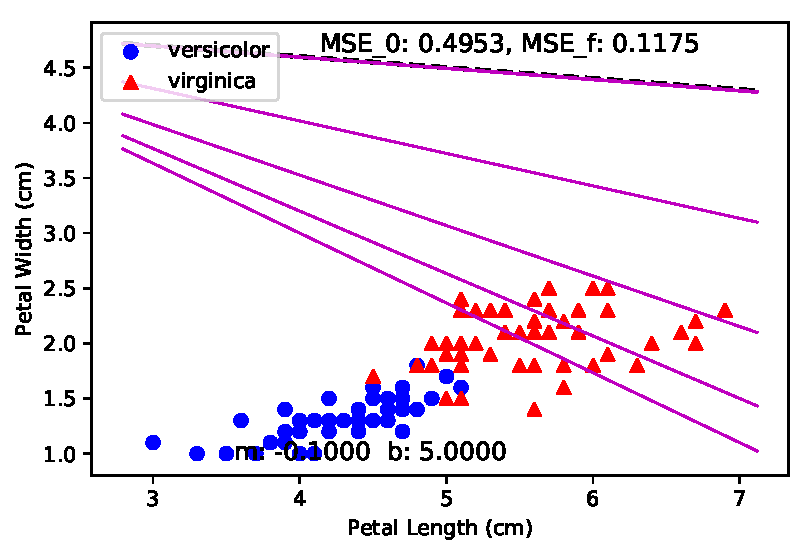
\includegraphics{plot_2e_1.pdf}
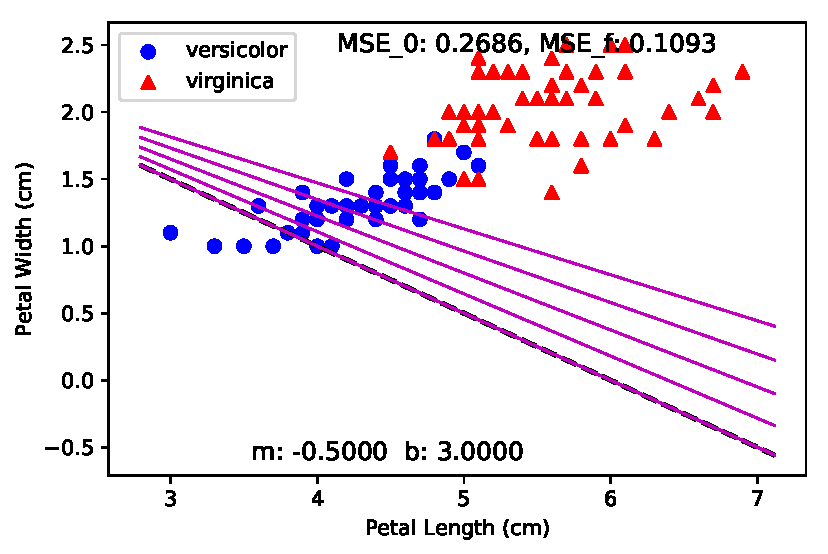
\includegraphics{plot_2e_2.pdf}
\end{center}

\section{Learning a Decision Boundary Through Optimization}

\subsection{Implementing Gradient Descent}

This section is basically the one above, since in the above plots I considered
it more helpful to show multiple steps at once. However since this section
covers the gradient descent implementation, I will point out that on the
previous graphs we notice initial and final MSE values, also reproduced
in the table below. The final value comes after 1000 steps, though not all
steps are always necessary.
\begin{center}
\begin{tabular}{|r|r|r|}
\hline
Initial MSE & Final MSE & Reduction\\
\hline\hline
0.4953 & 0.1175 & 76.3\%\\
\hline
0.2586 & 0.1093 & 57.7\%\\
\hline
\end{tabular}
\end{center}

We can also take a look at the descent function.
\begin{verbatim}
mse_0 = mean_squared_error(combined_data, slope, intercept)
m = slope
b = intercept
steps = 1000
for i in range(steps):
    m, b = sum_gradient(combined_data, m, b)
    if (i == 1) or (i % (steps / snapshots) == 0):
        # x_vals = np.array(ax.get_xlim())
        y_vals = b + m * x_vals
        plt.plot(x_vals, y_vals, color="m", linestyle='-', linewidth=1)
mse_f = mean_squared_error(combined_data, m, b)
\end{verbatim}
First the mean squared error is calculated for the inital weights. This is
$\text{MSE}_0$. Then we take $1000$ steps, and for every step a new gradient sum is
calculated, $m$ and $b$ are updated and plotted. After the $1000^{\text{th}}$
step, we calculated mean squared error once more. This is $\text{MSE}_f$.

The main point here is that there can be a significant reduction in MSE by
gradient descent.

\subsection{Showing the Learning Curve}

Now let us look at a learning curve for the first descent plot. This time it
is shown with a 100 steps visible, rather than just 5. You can see how the steps
``slow down'' as the boundary converges. Plus it might make a cool Moiré pattern
on your screen.
\begin{center}
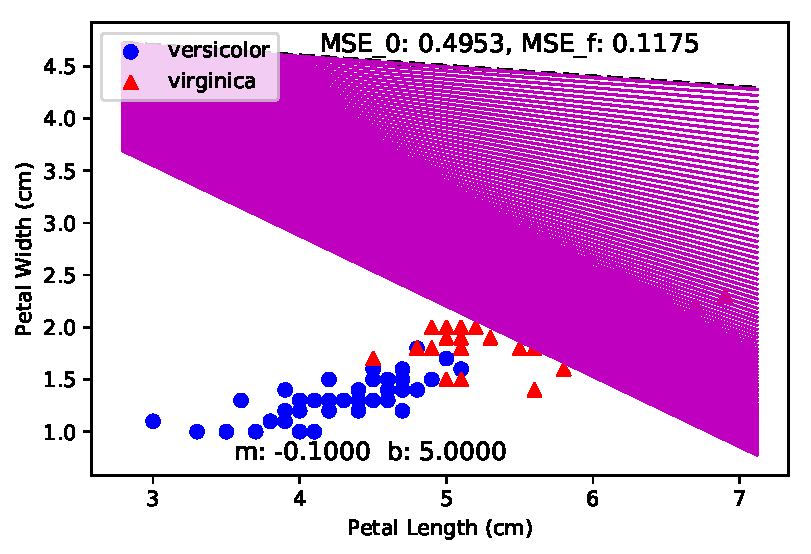
\includegraphics{plot_3b_1.pdf}
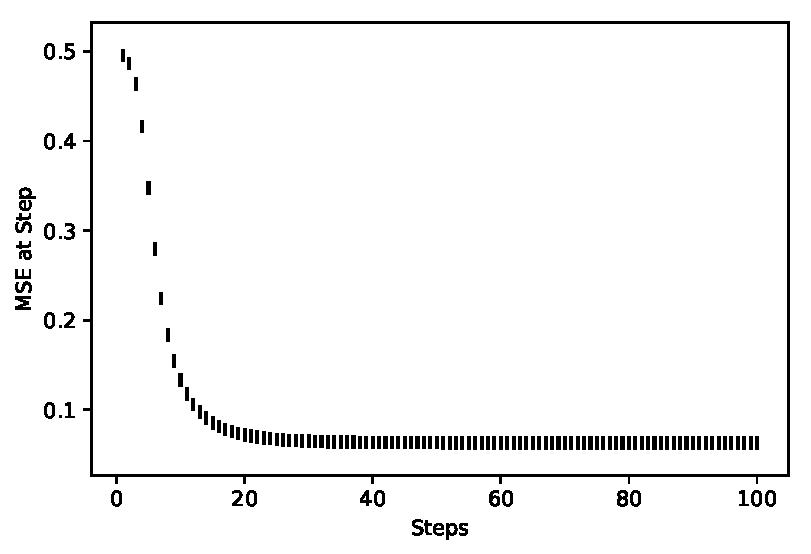
\includegraphics{plot_3b_2.pdf}
\end{center}
The learning curve is shown above.
\begin{verbatim}
mse_vals = []
m = slope
b = intercept
steps = 10000
for i in range(steps):
    if i % 100 == 0:
        mse_vals.append(mean_squared_error(dataset, m, b))
    m, b = sum_gradient(dataset, m, b)

fig = plt.figure()
ax = fig.add_subplot(111)
# mse_vals = mse_vals[int(-len(mse_vals)/2):]
ax.scatter(x=list(range(1, len(mse_vals) + 1)), y=mse_vals, color="k", marker="|")
plt.xlabel("Steps")
plt.ylabel("MSE at Step")
plt.savefig(filename, bbox_inches="tight")
plt.close(fig)
\end{verbatim}

\subsection{Illustration with Random Weights}

\subsection{Choosing the Gradient Step Size}
\subsection{Choosing the Stopping Criterion}

\end{document}